

\chapter{Métodos para Sistemas Não Lineares}\label{cap_snl}

Neste capítulo, estudamos sobre \hl{métodos para a resolução} de sistemas de equações não lineares. Vamos tratar o caso \hl{de problemas da forma}: encontrar $\pmb{x}\in\mathbb{R}^n$ tal que
\begin{equation}\hleq
  F(\pmb{x}) = \pmb{0},
\end{equation}
onde $F:\mathbb{R}^n\to\mathbb{R}^n$ é uma dada função vetorial.

\section{Método de Newton}\label{cap_snl_sec_newton}

Consideramos o problema de encontrar
\begin{equation}
  \pmb{x} = (x_1, x_2, \dotsc, x_n)\in\mathbb{R}^n
\end{equation}
tal que
\begin{equation}\label{cap_snl_sec_newton:eq:prob0}\hleq
  F(\pmb{x}) = \pmb{0},
\end{equation}
onde $F:\mathbb{R}^n\to\mathbb{R}^n$ é uma dada função vetorial com
\begin{equation}
  F(\pmb{x}) = (f_1(\pmb{x}), f_2(\pmb{x}), \dotsc, f_n(\pmb{x}))\in\mathbb{R}^n.
\end{equation}

Sejam \hl{$\pmb{x}^*$ a solução exata} de \eqref{cap_snl_sec_newton:eq:prob0} e \hl{$\pmb{x}^{(0)}$ uma dada aproximação de $\pmb{x}^*$}. Assim sendo, tomamos a seguinte \hl{expansão de $F$ em polinômio de Taylor}{\taylor}:
\begin{equation}\hleq
  F(\pmb{x}^*) = F(\pmb{x}^{(0)}) + J_F(\pmb{x}^{(0)})(\pmb{x}^*-\pmb{x}^{(0)}) + \pmb{r},
\end{equation}
onde $J_F$ é a \hl{\emph{matriz jacobiana}{\jacobi} de $F$}
\begin{align}
  \hleq{J_F(\pmb{x})} &:= \frac{\p(f_1, f_2, \dotsc, f_n)}{\p(x_1, x_2, \dotsc, x_n)}\\
  &\hleq{:= \begin{bmatrix}
    \frac{\p f_1}{\p x_1} & \frac{\p f_1}{\p x_2} & \ldots & \frac{\p f_1}{\p x_n}\\
    \frac{\p f_2}{\p x_1} & \frac{\p f_2}{\p x_2} & \ldots & \frac{\p f_2}{\p x_n}\\
    \vdots & \vdots & \vdots & \vdots \\
    \frac{\p f_n}{\p x_1} & \frac{\p f_n}{\p x_2} & \ldots & \frac{\p f_n}{\p x_n}\\
  \end{bmatrix}}
\end{align}
e $\|\pmb{r}\|^2\to 0$ quando $\|\pmb{x}^{(0)}-\pmb{x}^*\|\to 0$. 

Daí, como $F(\pmb{x}^*) = \pmb{0}$, segue que
\begin{equation}
  J_F(\pmb{x}^{(0)})(\pmb{x}^*-\pmb{x}^{(0)}) \approx -F(\pmb{x}^{(0)}).
\end{equation}
Então, multiplicando a inversa da jacobiana à esquerda, obtemos
\begin{equation}
  \pmb{x}^*-\pmb{x}^{(0)} \approx - J_F^{-1}(\pmb{x}^{(0)})F(\pmb{x}^{(0)})
\end{equation}
e, também,
\begin{equation}
  \pmb{x}^* \approx \pmb{x}^{(0)} - J_F^{-1}(\pmb{x}^{(0)})F(\pmb{x}^{(0)}).
\end{equation}

O exposto acima nos motiva a \hl{\emph{iteração de Newton}}{\newton}:
\begin{subequations}\hleq
  \begin{align}
    &\pmb{x}^{(0)} = \text{aprox. inicial},\\
    &\pmb{x}^{(k+1)} = \pmb{x}^{(k)} - J_F^{-1}(\pmb{x}^{(k)})F(\pmb{x}^{(k)}),
  \end{align}
\end{subequations}
com $k=0, 1, 2, \ldots$.

\begin{ex}\label{cap_snl_sec_newton:ex:newton_intro}
  Seja o sistema de equações não lineares
  \begin{subequations}
    \begin{align}
      & x_1x_2^2 = x_1^2x_2 - 6,\\
      & x_1^2x_2^3 - 7 = -x_1.
    \end{align}
  \end{subequations}
  Para usarmos o método de Newton, reescrevemos o sistema na seguinte forma
  \begin{subequations}
    \begin{align}
      x_1x_2^2 - x_1^2x_2 + 6 &= 0,\\
      x_1 + x_1^2x_2^3 - 7 &= 0.
    \end{align}
\end{subequations}
  Com isso, identificamos a função objetivo
  \begin{align}
    F(\pmb{x}) &=
    \begin{bmatrix}
      f_1(\pmb{x})\\
      f_2(\pmb{x})
    \end{bmatrix}\\
    &=
    \begin{bmatrix}
      x_1x_2^2 - x_1^2x_2 + 6\\
      x_1 + x_1^2x_2^3 - 7
    \end{bmatrix}
  \end{align}
  e calculamos sua matriz jacobiana
  \begin{align}
    J_F(\pmb{x}) &= \frac{\p(f_1, f_2)}{\p(x_1, x_2)} \\
                 &=
                   \begin{bmatrix}
                     \frac{\p f_1}{\p x_1} & \frac{\p f_1}{\p x_2}\\
                     \frac{\p f_2}{\p x_1} & \frac{\p f_2}{\p x_2}\\
                   \end{bmatrix}\\
                 &=
                   \begin{bmatrix}
                     x_2^2 - 2x_1x_2 & 2x_1x_2-x_1^2\\
                     1+2x_1x_2^3 & 3x_1^2x_2^2
                   \end{bmatrix}
  \end{align}
  Definidas $F$ e $J_F$ e tomando a aproximação inicial
  \begin{equation}
    \pmb{x}^{(0)} = (-1.5, 1.5)
  \end{equation}
  computamos as iterações de Newton e obtemos os resultados apresentados na Tabela \ref{cap_snl_sec_newton:tab:newton_intro}.

  \begin{table}[H]
    \centering
    \caption{Resultados referentes ao Exemplo \ref{cap_snl_sec_newton:ex:newton_intro}.}
    \begin{tabular}{lcc}\toprule
      k & $\pmb{x}^{(k)}$ & $\|F(\pmb{x}^{(k)})\|$\\\midrule
      0 & $(-1.50, 1.50)$ & $1.2\E+0$\\
      1 & $(-1.07, 1.82)$ & $1.2\E+0$\\
      2 & $(-9.95\E-1, 2.00)$ & $7.6\E-2$\\
      3 & $(-1.00, 2.00)$ & $1.2\E-4$ \\
      4 & $(-1.00, 2.00)$ & $2.1\E-9$ \\\bottomrule
    \end{tabular}
    \label{cap_snl_sec_newton:tab:newton_intro}
  \end{table}

\begin{lstlisting}
import numpy as np
import numpy.linalg as npla

def newton(F, J, x0, 
           maxiter=100, tol=1.49e-8):
  print(f'\n{0}: x = {x0}, ' + \
        f'norm = {npla.norm(F(x0)):.1e}')
  info = -1
  for k in range(maxiter):
    x = x0 - npla.inv(J(x0))@F(x0)
    print(f'{k+1}: x = {x}, ' + \
          f'norm = {npla.norm(F(x)):.1e}')
    if (npla.norm(x - x0) < tol):
      info = 0
      break
    x0 = x.copy()
  return x, info

def F(x):
  n = x.size
  y = np.empty(n)
  y[0] = x[0]*x[1]**2 - x[0]**2*x[1] + 6
  y[1] = x[0] + x[0]**2*x[1]**3 - 7
  return y

def J(x):
  n = x.size
  y = np.empty((n,n))
  y[0,0] = x[1]**2 - 2*x[0]*x[1]
  y[0,1] = 2*x[0]*x[1] - x[0]**2
  y[1,0] = 1 + 2*x[0]*x[1]**3
  y[1,1] = 3*x[0]**2*x[1]**2
  return y

x0 = np.array([-1.5, 1.5])
x, info = newton(F, J, x0)
\end{lstlisting}

\end{ex}

\subsection{Análise Numérica}

Para uma função $F$ suficientemente suave e com uma escolha apropriada da aproximação inicial $\pmb{x}^{(0)}$, temos que as \hl{iterações de Newton}
\begin{equation}
  \pmb{x}^{(k+1)} = \pmb{x}^{(k)} - J_F^{-1}(\pmb{x}^{(k)})F(\pmb{x}^{(k)}),
\end{equation}
com $k=0, 1, 2, \ldots$, \hl{são quadraticamente convergentes}\endnote{Para informações mais precisas sobre a convergência do Método de Newton, consulte \cite[Seção 5.3]{Stoer1993a}.}, i.e.
\begin{equation}\hleq
  \|\pmb{x}^{(k+1)} - \pmb{x}^*\| \leq C\|\pmb{x}^{(k)}-\pmb{x}^*\|^2,
\end{equation}
onde $\pmb{x}^*$ é a solução exata, i.e. $F(\pmb{x}^*) = \pmb{0}$.

\begin{ex}\label{cap_snl_sec_newton:ex:newton_conv}
  Consideremos o seguinte sistema de equações não lineares
  \begin{align}
    x_1x_2^2 - x_1^2x_2 + 6 &= 0,\\
    x_1 + x_1^2x_2^3 - 7 &= 0.
  \end{align}
  A Figura \ref{cap_snl_sec_newton:fig:ex_newton_conv} é um esboço do gráfico da $\|F(\cdot)\|$. Este problema foi confeccionado de forma que $\pmb{x}^* = (-1, 2)$. Então, tomando $\pmb{x}^{(0)} = (1.5, 1.5)$ como aproximação inicial, computamos as iterações de Newton para este problema, donde obtemos os resultados reportados na Tabela \ref{cap_snl_sec_newton:tab:ex_newton_conv}. 

  \begin{figure}[h!]
    \centering
    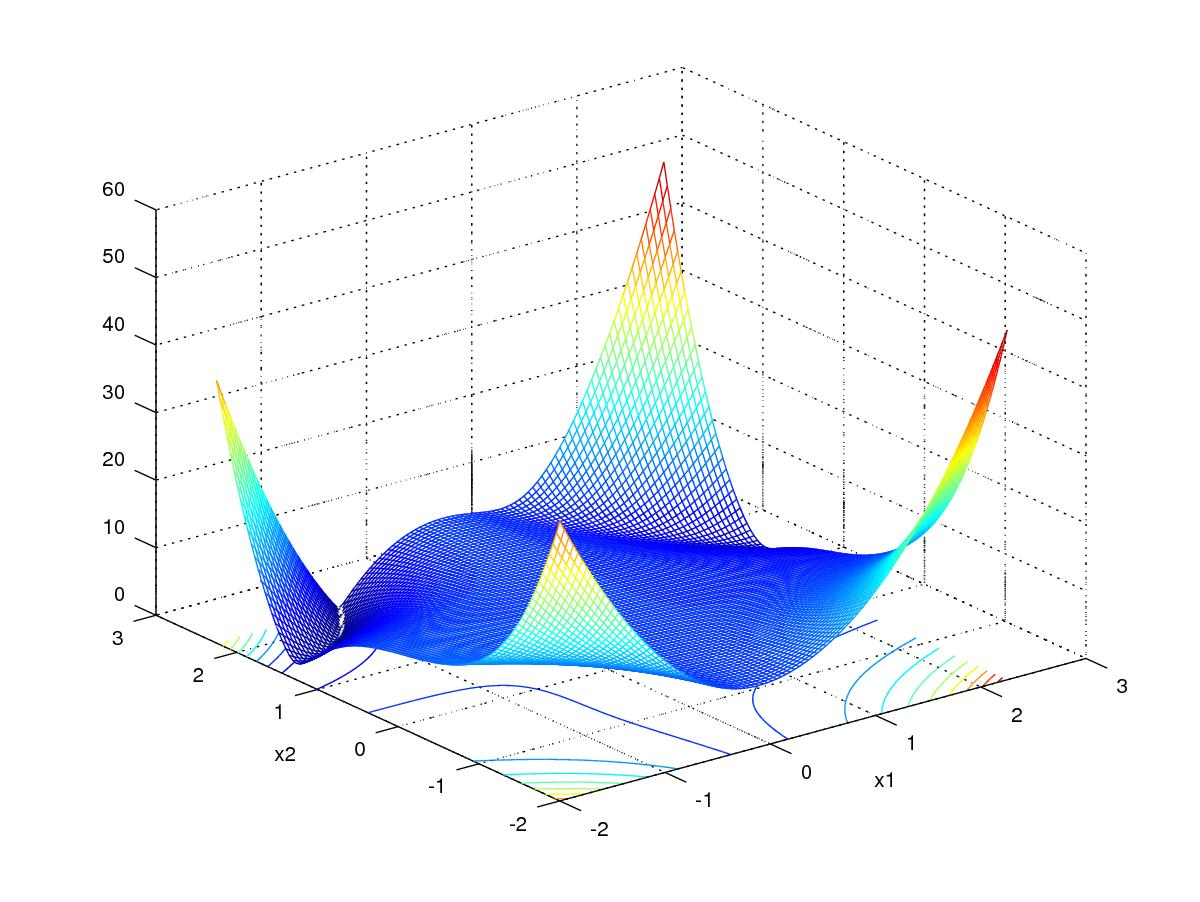
\includegraphics[width=0.7\textwidth]{./cap_snl/dados/ex_newton_conv/ex_newton_conv}
    \caption{Esboço do gráfico de $\|F(\cdot)\|$ referente ao Exemplo \ref{cap_snl_sec_newton:ex:newton_conv}.}
    \label{cap_snl_sec_newton:fig:ex_newton_conv}
  \end{figure}

  \begin{table}[H]
    \centering
    \begin{tabular}{lcc}
      k & $\pmb{x}^{(k)}$ & $\|\pmb{x}^{(k)} - \pmb{x}^*\|$\\\hline
      0 & $(-1.50, 1.50)$ & $7.1\E-01$\\
      1 & $(-1.07, 1.82)$ & $2.0\E-01$\\
      2 & $(-9.95\E-1, 2.00)$ & $5.1\E-03$\\
      3 & $(-1.00, 2.00)$ & $2.6\E-05$ \\
      4 & $(-1.00, 2.00)$ & $2.0\E-10$ \\
      5 & $(-1.00, 2.00)$ & $3.1\E-16$ \\\hline
    \end{tabular}
    \caption{Resultados referentes ao Exemplo \ref{cap_snl_sec_newton:ex:newton_conv}.}
    \label{cap_snl_sec_newton:tab:ex_newton_conv}
  \end{table}
\end{ex}

\subsection{Exercícios}

\begin{exer}
  Use o Método de Newton para computar uma solução aproximada para o sistema de equações
  \begin{subequations}
    \begin{align}
      & \frac{x_1^2}{3} + x_2^2 = 1\\
      & x_1^2 + \frac{x_2^2}{4} = 1
    \end{align}
  \end{subequations}
\end{exer}
\begin{resp}
  Soluções exatas: $\pmb{x} = \pm\left(\sqrt{\frac{9}{11}}, \sqrt{\frac{8}{11}}\right)$.
\end{resp}

\begin{exer}
  Use o Método de Newton, com aproximação inicial $\pmb{x}^{(0)} = (1.5, 0.5)$ para computar uma solução aproximada para o sistema de equações
  \begin{subequations}
    \begin{align}
      & x_1^2 = \cos(x_1x_2) + 1\\
      & \sen(x_2) = 2\cos(x_1)
    \end{align}
  \end{subequations}
\end{exer}
\begin{resp}
  $\pmb{x} = (1.3468109, 0.4603195)$
\end{resp}

\begin{exer}
  Use o Método de Newton, com aproximação inicial $\pmb{x}^{(0)} = (1, -1)$ para computar uma solução aproximada para o sistema de equações
  \begin{subequations}
    \begin{align}
      & 3x_1 = \cos(x_1x_2) + \frac{1}{2}\\
      & 4x_1^2 + 2x_2x_1 = 0
    \end{align}
  \end{subequations}  
\end{exer}
\begin{resp}
  $\pmb{x} = (4.668417\E-1, -9.368334\E-1)$
\end{resp}

\begin{exer}
  Use o método de Newton para obter uma aproximação de uma solução de
  \begin{align}
    x_2\sen(x_3)+x_1-2&=0,\\
    x_1x_2-\sen(x_2)+0.2&=0,\\
    x_3^2+\cos(x_1x_2)-4.5&=0.
  \end{align}
Para tanto, use $\pmb{x}^{(1)} = (1, -1, -1)$.
\end{exer}
\begin{resp}
  $\pmb{x} = (1.7519\E+0, -2.6202\E-1, -1.8983\E+0)$
\end{resp}

\begin{exer}
  Considere o problema de encontrar os pontos de interseção no plano $x-y$ da elipse
  \begin{equation}
    \frac{x^2}{4} + \frac{y^2}{9} = 1
  \end{equation}
  com a curva
  \begin{equation}
    x = y^2\sqrt{x}.
  \end{equation}
  Escreva o problema na forma $F(\pmb{x}) = \pmb{0}$ e use o Método de Newton para encontrar o ponto de interseção próximo de $(x, y) = (1.5, 1.5)$.
\end{exer}
\begin{resp}
  $x = 1.842996\E+0$, $y = 1.165148\E+0$
\end{resp}

\ifisbook
\subsubsection{Respostas}
\shipoutAnswer
\fi

%%% SECTION %%%

\section{Métodos \textit{Quasi}-Newton}\label{cap_snl_sec_quasi_newton}
\badgeRevisar

\subsection{Método do Acorde}
\badgeRevisar

O método do acorde consiste na seguinte iteração
\begin{align}
  \pmb{x}^{(1)} &= \text{aprox. inicial},\\
  \pmb{x}^{(k+1)} &= \pmb{x}^{(k)} - J_F^{-1}(\pmb{x}^{(1)})F(\pmb{x}^{(k)}).
\end{align}
Ou seja, é a iteração de Newton com jacobina constante.

\begin{ex}\label{ex:acorde_exec}
  Consideremos o seguinte sistema de equações não lineares
  \begin{align}
    x_1x_2^2 - x_1^2x_2 + 6 &= 0,\\
    x_1 + x_1^2x_2^3 - 7 &= 0.
  \end{align}
  Definidas $F$ e $J_F$ e tomando $\pmb{x}^{(1)} = (1.5, 1.5)$ como aproximação inicial, computamos as iterações do método do acorde de forma a obtermos os resultados apresentados na Tabela \ref{tab:ex_acorde_exec}.

  \begin{table}[h!]
    \centering
    \begin{tabular}{lcc}
      k & $\pmb{x}^{(k)}$ & $\|\pmb{x}^{(k)} - \pmb{x}^*\|$\\\hline
      1 & $(-1.50, 1.50)$ & -x- \\
      2 & $(-1.07, 1.82)$ & $5.3\E-1$ \\
      3 & $(-1.02, 1.93)$ & $1.2\E-1$ \\
      4 & $(-1.00, 1.98)$ & $5.2\E-2$ \\
      5 & $(-9.98\E-1, 2.00)$ & $1.8\E-2$ \\
      6 & $(-9.98\E-1, 2.00)$ & $4.7\E-3$ \\
      7 & $(-9.99\E-1, 2.00)$ & $9.0\E-4$ \\
      8 & $(-1.00, 2.00)$ & $7.4\E-4$ \\
      9 & $(-1.00, 2.00)$ & $4.3\E-4$ \\\hline
    \end{tabular}
    \caption{Resultados referentes ao Exemplo \ref{ex:acorde_exec}.}
    \label{tab:ex_acorde_exec}
  \end{table}

% \ifisoctave
% No \verb+GNU Octave+, podemos fazer as computações acima com o seguinte \href{https://github.com/phkonzen/notas/blob/master/src/MatematicaNumerica/cap_snl/dados/ex_acorde_exec/ex_acorde_exec.m}{código}:
% \verbatiminput{./cap_snl/dados/ex_acorde_exec/ex_acorde_exec.m}
% \fi
\end{ex}

\subsection{Jacobiana Aproximada}
\badgeRevisar

A jacobiana $J_F(\pmb{x})$ de uma dada função $F(\pmb{x}) = (f_1(\pmb{x}), f_2(\pmb{x}), \dotsc, f_n(\pmb{x}))$ é a matriz cujo elemento da $i$-ésima linha e $j$-ésima coluna é
\begin{equation}
  \frac{\p f_i}{\p x_j} = \lim_{h\to 0} \frac{f_i(\pmb{x}+\pmb{e}_jh) - f_i(\pmb{x})}{h},
\end{equation}
onde $\pmb{e}_j$ é o $j$-ésimo vetor da base canônica de $\mathbb{R}^n$, i.e. $\pmb{e}_j = (0, \dotsc, 0, 1, 0, \dotsc, 0)$ com $1$ na $j$-ésima posição.

Com isso, podemos computar uma jacobiana aproximada tomando
\begin{equation}
  \frac{\p f_i}{\p x_j} \approx \frac{f_i(\pmb{x}+\pmb{e}_jh) - f_i(\pmb{x})}{h},
\end{equation}
com $h$ suficientemente pequeno.

\begin{ex}\label{ex:jacaprox_exec}
  Consideremos o seguinte sistema de equações não lineares
  \begin{align}
    x_1x_2^2 - x_1^2x_2 + 6 &= 0,\\
    x_1 + x_1^2x_2^3 - 7 &= 0.
  \end{align}
  Definida $F$, sua jacobina aproximada $\tilde{J}_F$ com $h=10^{-7}$ e tomando $\pmb{x}^{(1)} = (1.5, 1.5)$ como aproximação inicial, computamos as iterações do {\it quasi}-método de forma a obtermos os resultados apresentados na Tabela \ref{tab:ex_jacaprox_exec}.

  \begin{table}[h!]
    \centering
    \begin{tabular}{lcc}
      k & $\pmb{x}^{(k)}$ & $\|\pmb{x}^{(k)} - \pmb{x}^*\|$\\\hline
      1 & $(-1.50, 1.50)$ & -x- \\
      2 & $(-1.07, 1.82)$ & $5.3\E-1$\\
      3 & $(-9.95\E-1, 2.00)$ & $2.0\E-1$\\
      4 & $(-1.00, 2.00)$ & $5.1\E-3$\\
      5 & $(-1.00, 2.00)$ & $2.6\E-5$\\\hline
    \end{tabular}
    \caption{Resultados referentes ao Exemplo \ref{ex:jacaprox_exec}.}
    \label{tab:ex_jacaprox_exec}
  \end{table}

% \ifisoctave
% No \verb+GNU Octave+, podemos fazer as computações acima com o seguinte \href{https://github.com/phkonzen/notas/blob/master/src/MatematicaNumerica/cap_snl/dados/ex_jacaprox_exec/ex_jacaprox_exec.m}{código}:
% \verbatiminput{./cap_snl/dados/ex_jacaprox_exec/ex_jacaprox_exec.m}
% \fi
\end{ex}

\subsection{Exercícios}

\badgeConstrucao

\ifisbook
\subsubsection{Respostas}
\shipoutAnswer
\fi

%%% SECTION %%%